\documentclass[14 pt]{extarticle}
\usepackage[utf8]{inputenc} 
\usepackage[T1,T2A]{fontenc}
\usepackage[english, ukrainian]{babel}
\usepackage[center]{titlesec}
\usepackage{amsmath, amsfonts}
\usepackage{mathtools}
\usepackage{marvosym}
\usepackage{geometry}
\geometry{verbose,a4paper,tmargin=1.5cm,bmargin=1.5cm,lmargin=1.8cm,rmargin=2cm}
\usepackage{diagbox}
\usepackage{hyperref}
\usepackage{nicefrac}
\usepackage{graphicx}
\usepackage{pgfplots}
\usepackage{physics}
\usepackage{relsize}
\usepackage{textgreek}
\usepackage{upgreek}
\usepackage{adjustbox}
\usepackage{pdfpages}
\linespread{1.3}
\makeatletter
\renewcommand*\env@matrix[1][\arraystretch]{%
  \edef\arraystretch{#1}%
  \hskip -\arraycolsep
  \let\@ifnextchar\new@ifnextchar
  \array{*\c@MaxMatrixCols c}}
\makeatother

\usepgfplotslibrary{fillbetween}
\usepackage{float}
\hypersetup{
    colorlinks=true,
    linkcolor = blue,
}
\DeclareMathOperator*{\argmax}{argmax} % thin space, limits underneath in displays
\usepackage{tikz}
\newcommand*\circled[1]{\tikz[baseline=(char.base)]{
            \node[shape=circle,draw,inner sep=2pt] (char) {#1};}}

            


\begin{document}



\begin{titlepage}
    \begin{center}
        
        
\includegraphics[width=18cm]{image1.png}
        Мiнiстерство освiти i науки України \\
        Національний технічний університет України \\
        «Київський політехнічний інститут імені Ігоря Сікорського» Iнститут прикладного системного аналiзу \\

        \vspace{4.5cm}
        \textbf{Лабораторна робота № 3}\\
        з курсу «Чисельнi методи» \\
        з теми «Методи розв'язання нелінійних систем» \\
        Варіант № 9 \\
    \end{center}

    \vspace{2cm}

    \begin{flushright}
        Виконав студент 2 курсу групи КА-02 \\
        Романович Володимир Володимирович \\
        перевiрила старший викладач \\
        Хоменко Ольга Володимирiвна \\

    \end{flushright}

    \vfill
    \begin{center}
        Київ -- 2022
    \end{center}
\end{titlepage}


\begin{center}
    \large
    \textbf{Задача 1}
\end{center}
$
\begin{cases}
\cos{(x+0.5)} - y = 2 \\
\sin{y} - 2x = 1
\end{cases}
$
\\ 
Запишемо систему у вигляді $\vec{x} = \Phi(\vec{x})$: \\ 
$
\begin{cases}
x = \frac12 (\sin{y}-1)\\
y=\cos{(x+0.5)} - 2
\end{cases} \implies
 \vec{x} =
\begin{pmatrix}
x \\ y
\end{pmatrix} =
\begin{pmatrix}
\frac12 (\sin{y}-1) \\
\cos{(x+0.5)} - 2
\end{pmatrix} = \Phi(\vec{x})
$ \\ 
Побудуємо графік для знаходження початкового наближення:\\ 
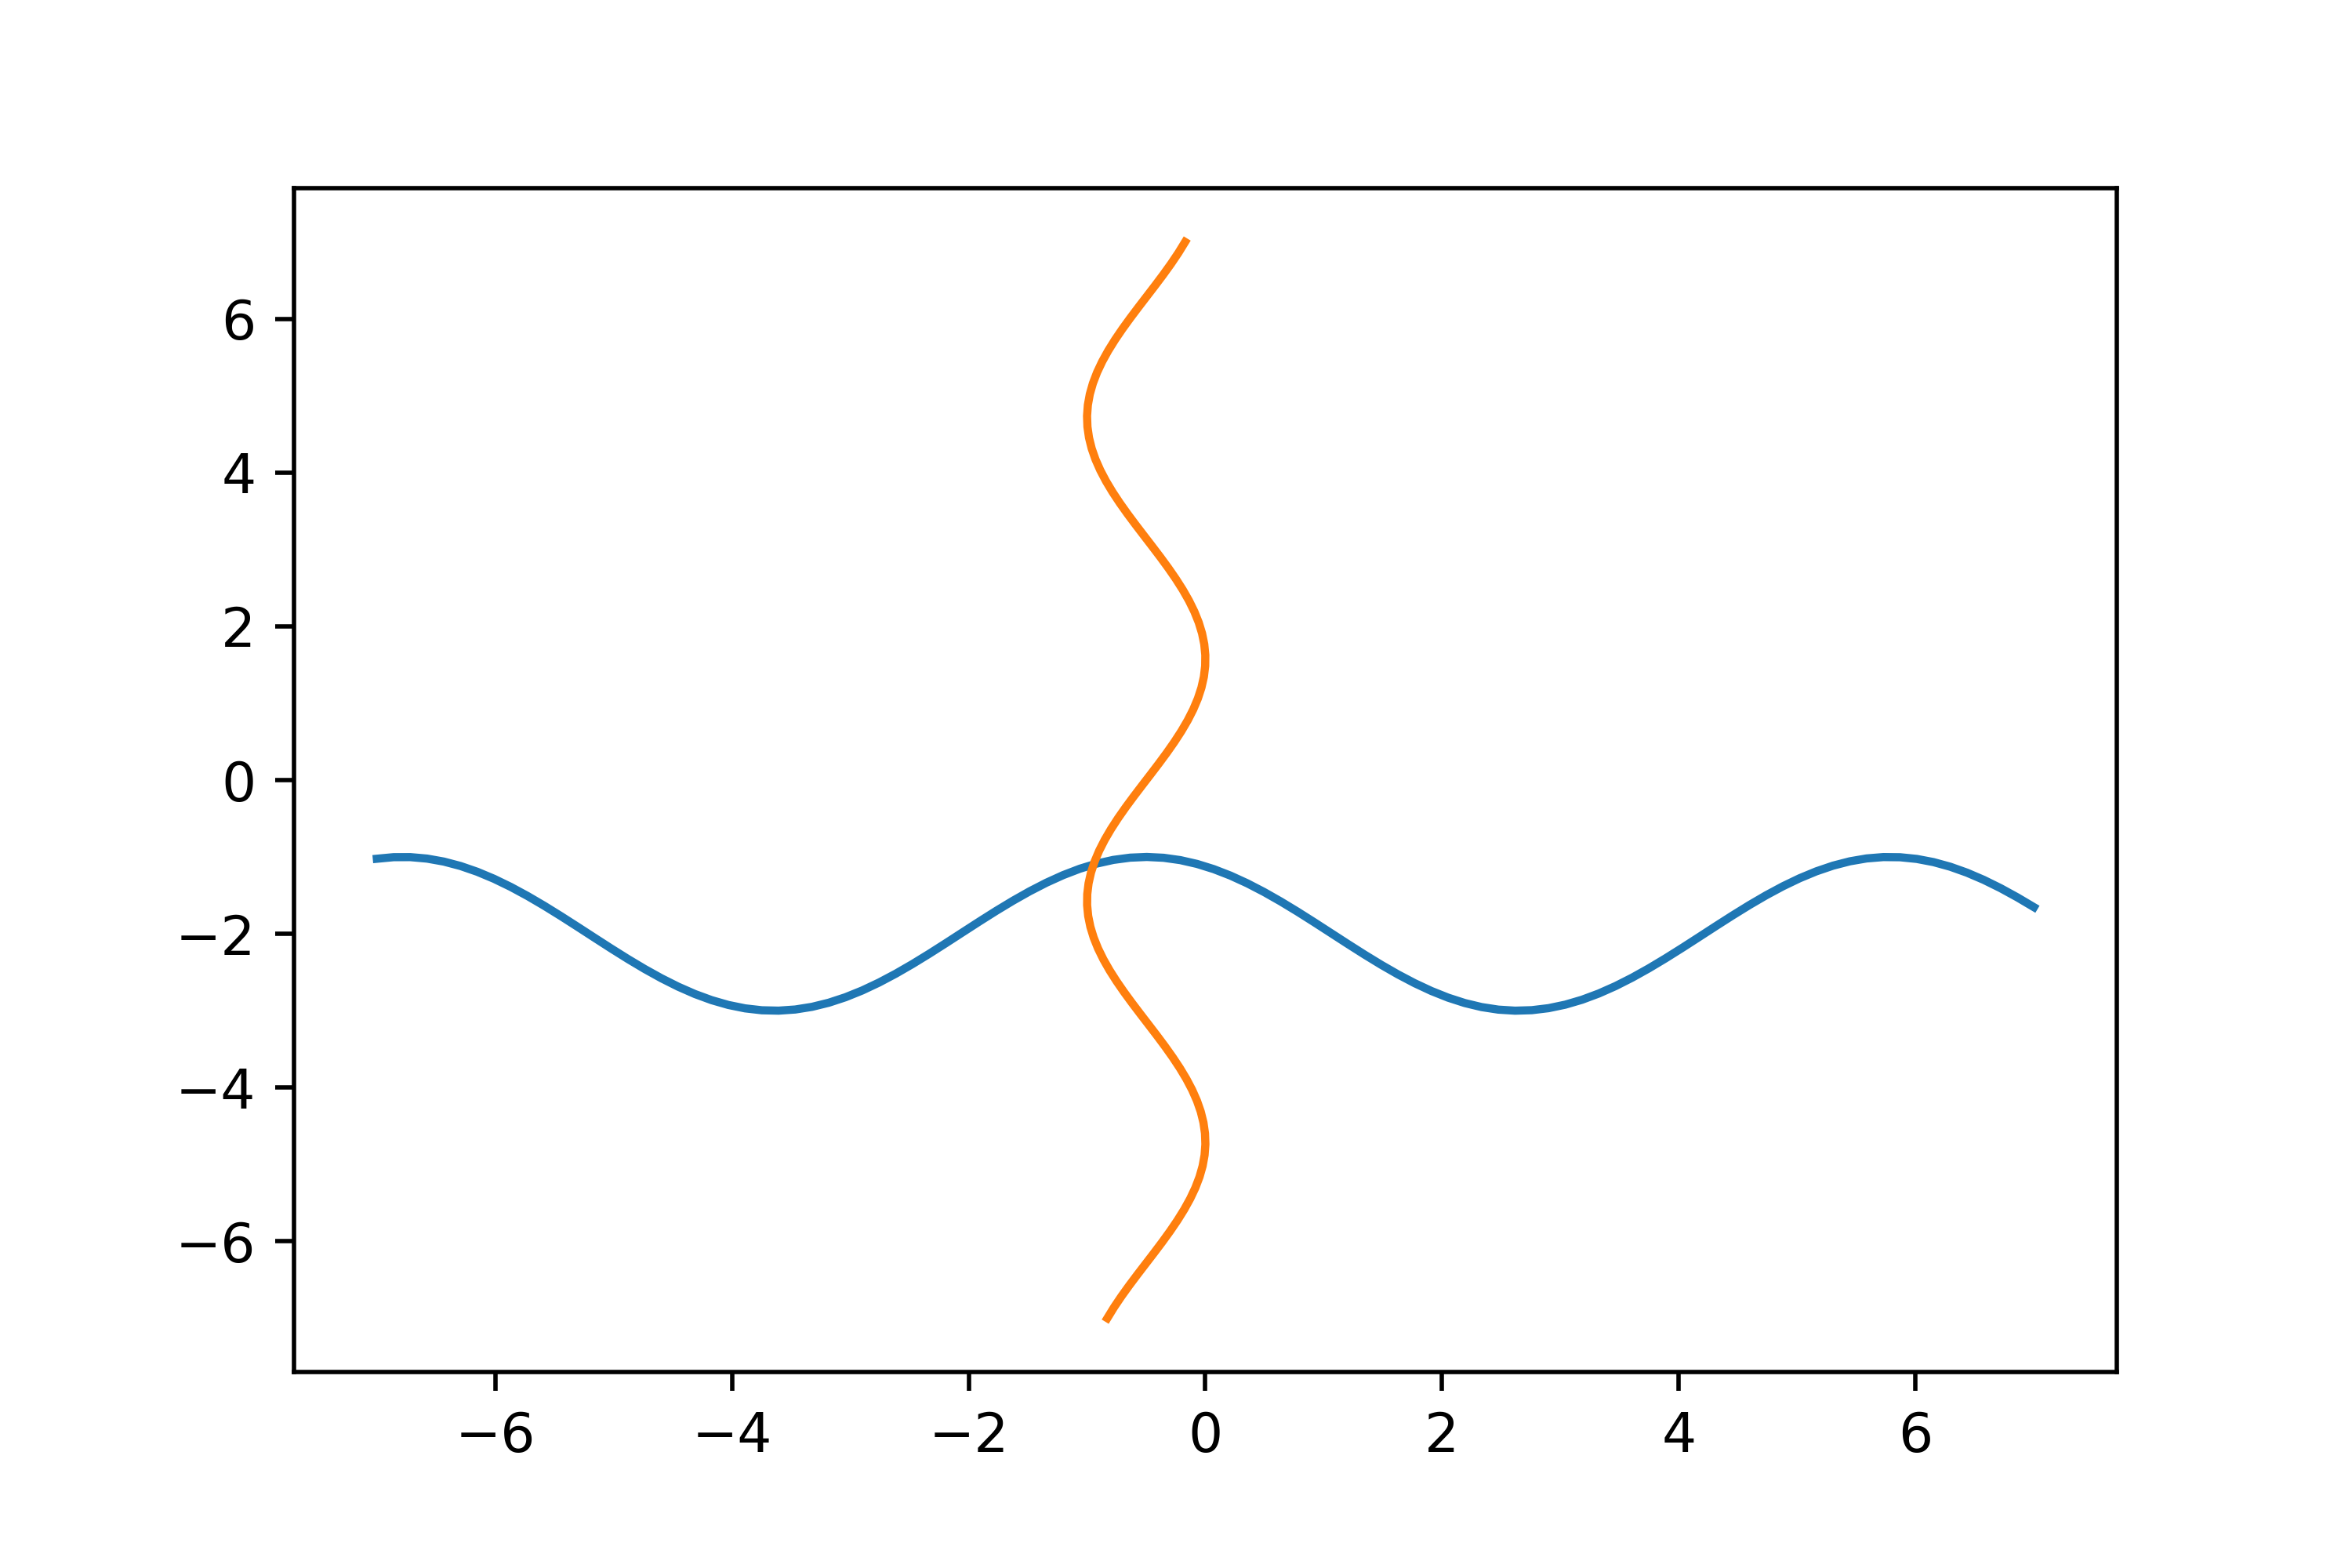
\includegraphics[width=12cm]{plot.png}
\ \\ 
Перевіримо достатню умову збіжності\\ 
Нехай G = $\{ |x + 1| \leq 0.2, |y + 1| \leq 0.2 \}$ \\ 
$\frac{\partial \varphi_1}{\partial x } =  0$, \ \ \ 
$\frac{\partial \varphi_1}{\partial y } =  \frac{1}{2} \cos{y}$ \\ 
$\frac{\partial \varphi_2}{\partial x } =  - \sin{(x+0.5)}$, \ \ \  
$\frac{\partial \varphi_2}{\partial y } =  0$ \\
$$
\left| \frac{\partial \varphi_1}{\partial x } \right| 
+ \left| \frac{\partial \varphi_2}{\partial x } \right| 
= |\sin{(x+0.5)}| \leq |\sin{(-1.2+0.5)}| \leq 0.65 < 1
$$
$$
\left| \frac{\partial \varphi_1}{\partial y } \right| 
+ \left| \frac{\partial \varphi_2}{\partial y } \right| 
= \left|\frac{1}{2} \cos{y}\right|\leq 0.5 < 1
$$
Отже якщо послідовні наближення не будуть виходити за G то ітераційний процес збіжний і розв'язок єдиний. \\ 
Запрограмувавши метод простих ітерацій отримали розв'язок: \\ 
\begin{tabular}{|c|c|c|c|} \hline
    Iter & x & y & $\Delta$ \\ \hline
    0 & -1.000000 & -1.000000 &   \\ \hline
    1 & -0.920735 & -1.122417 & 0.122417 \\\hline
    2 & -0.950576 & -1.087211 & 0.035206 \\\hline
    3 & -0.942667 & -1.099803 & 0.012592 \\\hline
    4 & -0.945559 & -1.096387 & 0.003416 \\\hline
    5 & -0.944781 & -1.097630 & 0.001243 \\\hline
    6 & -0.945065 & -1.097295 & 0.000335 \\\hline
    7 & -0.944989 & -1.097417 & 0.000122 \\\hline
    8 & -0.945016 & -1.097384 & 0.000033 \\\hline
    9 & -0.945009 & -1.097396 & 0.000012 \\\hline
    10 & -0.945012 & -1.097393 & 0.000003 \\\hline
    \end{tabular} \\ 
Також взявши інші початкові наближення ми отримуємо такий же результат(з точністю до $\varepsilon$),
але можливо з більшою кількістю ітерацій. Наприклад наведемо таблицю з початковим наближенням (500, -500): \\ 
\begin{tabular}{|c|c|c|c|}\hline
   Iter & x & y & $\Delta$ \\\hline
   0 & 500.000000 & -500.000000 &   \\\hline
   1 & -0.266114 & -2.551389 & 500.266114 \\\hline
   2 & -0.778265 & -1.027227 & 1.524162 \\\hline
   3 & -0.927934 & -1.038467 & 0.149669 \\\hline
   4 & -0.930813 & -1.090175 & 0.051708 \\\hline
   5 & -0.943354 & -1.091374 & 0.012540 \\\hline
   6 & -0.943631 & -1.096682 & 0.005308 \\\hline
   7 & -0.944849 & -1.096801 & 0.001218 \\\hline
   8 & -0.944876 & -1.097324 & 0.000523 \\\hline
   9 & -0.944995 & -1.097336 & 0.000119 \\\hline
   10 & -0.944998 & -1.097387 & 0.000051 \\\hline
   11 & -0.945010 & -1.097388 & 0.000012 \\\hline
   12 & -0.945010 & -1.097393 & 0.000005 \\\hline
   \end{tabular}\\ 
Отже отримали розв'язок $(x,y) = (-0.94501;-1.09739)$ 
 \newpage 
 \begin{center}
    \Large
    Задача 2
\end{center}
Розв'язати систему рівнянь $
\begin{cases}
tg(xy) = x^2 \\
0.7x^2 + 2y^2 = 1
\end{cases}
$ спрощеним методом Ньютона. 
$f_1 (\vec{x}) = tg(xy) - x^2 = 0, \ \ \ f_2 (\vec{x}) = 0.7x^2+2y^2-1=0$ 
$$
W = \begin{pmatrix}
    \frac{\partial f_1}{\partial x} & \frac{\partial f_1}{\partial y} \\ 
    \frac{\partial f_2}{\partial x} & \frac{\partial f_2}{\partial y}
\end{pmatrix} = 
\begin{pmatrix}
    \frac{y}{\cos^2(xy)} - 2x & \frac{x}{\cos^2(xy)} \\ 
    1.4x & 4y 
\end{pmatrix}
$$
$$
F = \begin{pmatrix}
    tg(xy) - x^2 \\ 
    0.7x^2+2y^2-1
\end{pmatrix}
$$
Побудуємо графік для знаходження початкового наближення: \\ 
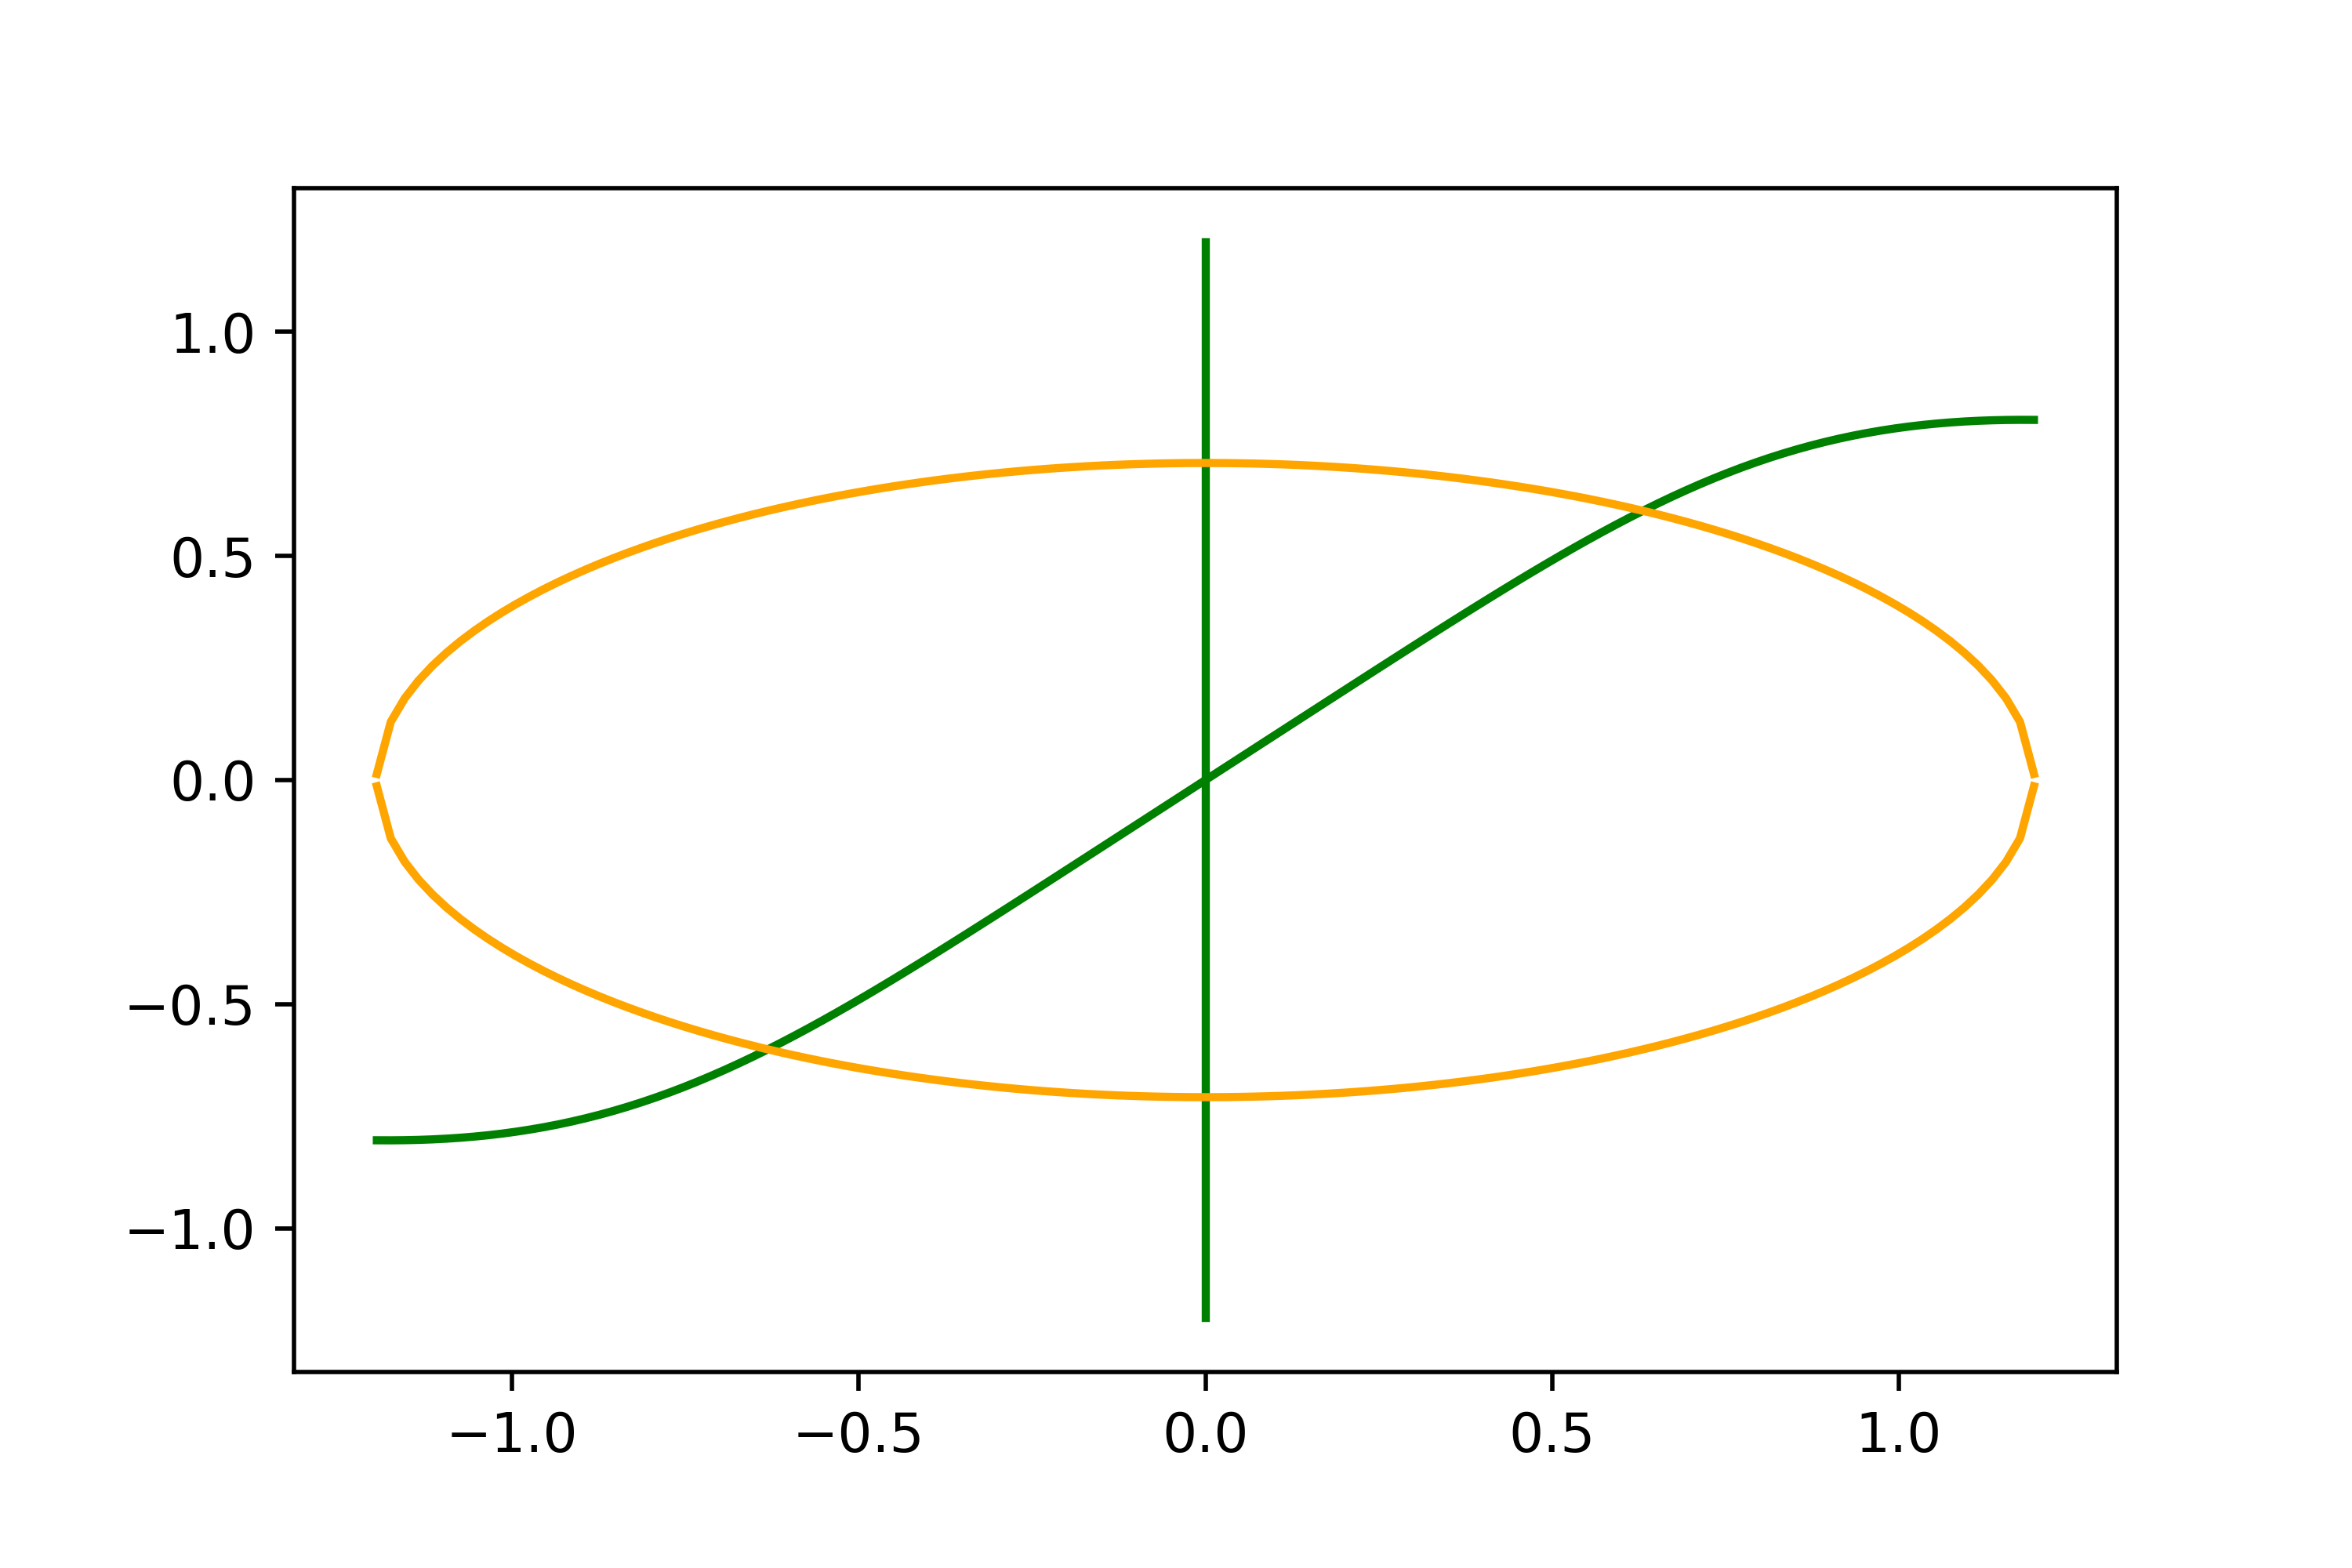
\includegraphics[width=12cm]{plot2.png} \\ 
Бачимо що графіки мають 4 точки перетину, оберемо для цих точок початкові наближення: 
(0.6, 0.6), (0, 0.7), (-0.6, -0.6), (0, -0.7) \\ 
Запрограмувавши спрощений метод Ньютона, отримали такі розв'язки: \\ 
(0.63103, 0.60053) (0, 0.70711) (-0.63103, -0.60053) (0, -0.70711)\\
Для розв'язку (0.63103, 0.60053) наведемо таблицю із значеннями x,y,$\Delta$ на кожній ітерації: \\ 
\begin{tabular}{|c|c|c|c|} \hline
    Iter & x & y & $\Delta$ \\ \hline
    0 & 0.600000 & 0.600000 &   \\ \hline
    1 & 0.632322 & 0.600354 & 0.032322 \\ \hline
    2 & 0.630903 & 0.600546 & 0.001419 \\ \hline
    3 & 0.631037 & 0.600525 & 0.000134 \\ \hline
    4 & 0.631024 & 0.600527 & 0.000013 \\ \hline
    5 & 0.631025 & 0.600527 & 0.000001 \\ \hline
\end{tabular} \\ 
Задавши початкове наближення (100, 200) ми не отримали розв'язок за 999 ітерацій та, скоріш за все,
метод не є збіжним при такому початковому наближенні. \\ 
Також була проведена перевірка за допомогою функції fsolve() та обчисленням $F(\vec{x}_*)$,
де $\vec{x}_*$ -- знайдений розв'язок. Отримали що з точністю $\varepsilon$
наш розв'язок дорівнює розв'язку з fsolve() та $F(\vec{x}_*) = \vec{0}$    
\begin{center}
    \Large
    Висновки
\end{center}
Мовою програмування Python ми реалізували методи простих ітерацій та спрощений метод Ньютона
для розв'язку нелінійних систем рівнянь, побудувавши графік знайшли початкові наближення
та підставивши ці наближення в функції, отримали правильний(перевірений декількома способами)
розв'язок. У випадку методу простих ітерацій із зміною початкового наближення відповідь
не змінилась, проте збільшилась кількість ітерацій, а у випадку спрощеного методу Ньютона,
через те що він тільки локально збіжний, ми не змогли отримати розв'язок з наближенням (100, 200). 
Це не дивно, оскільки область збіжності цього методу є досить малою, і потрібно обирати
початкове наближення близьке до розв'язку, як ми це і зробили після побудови графіку. \\ 
Лістинг програми наведений знизу \\ 
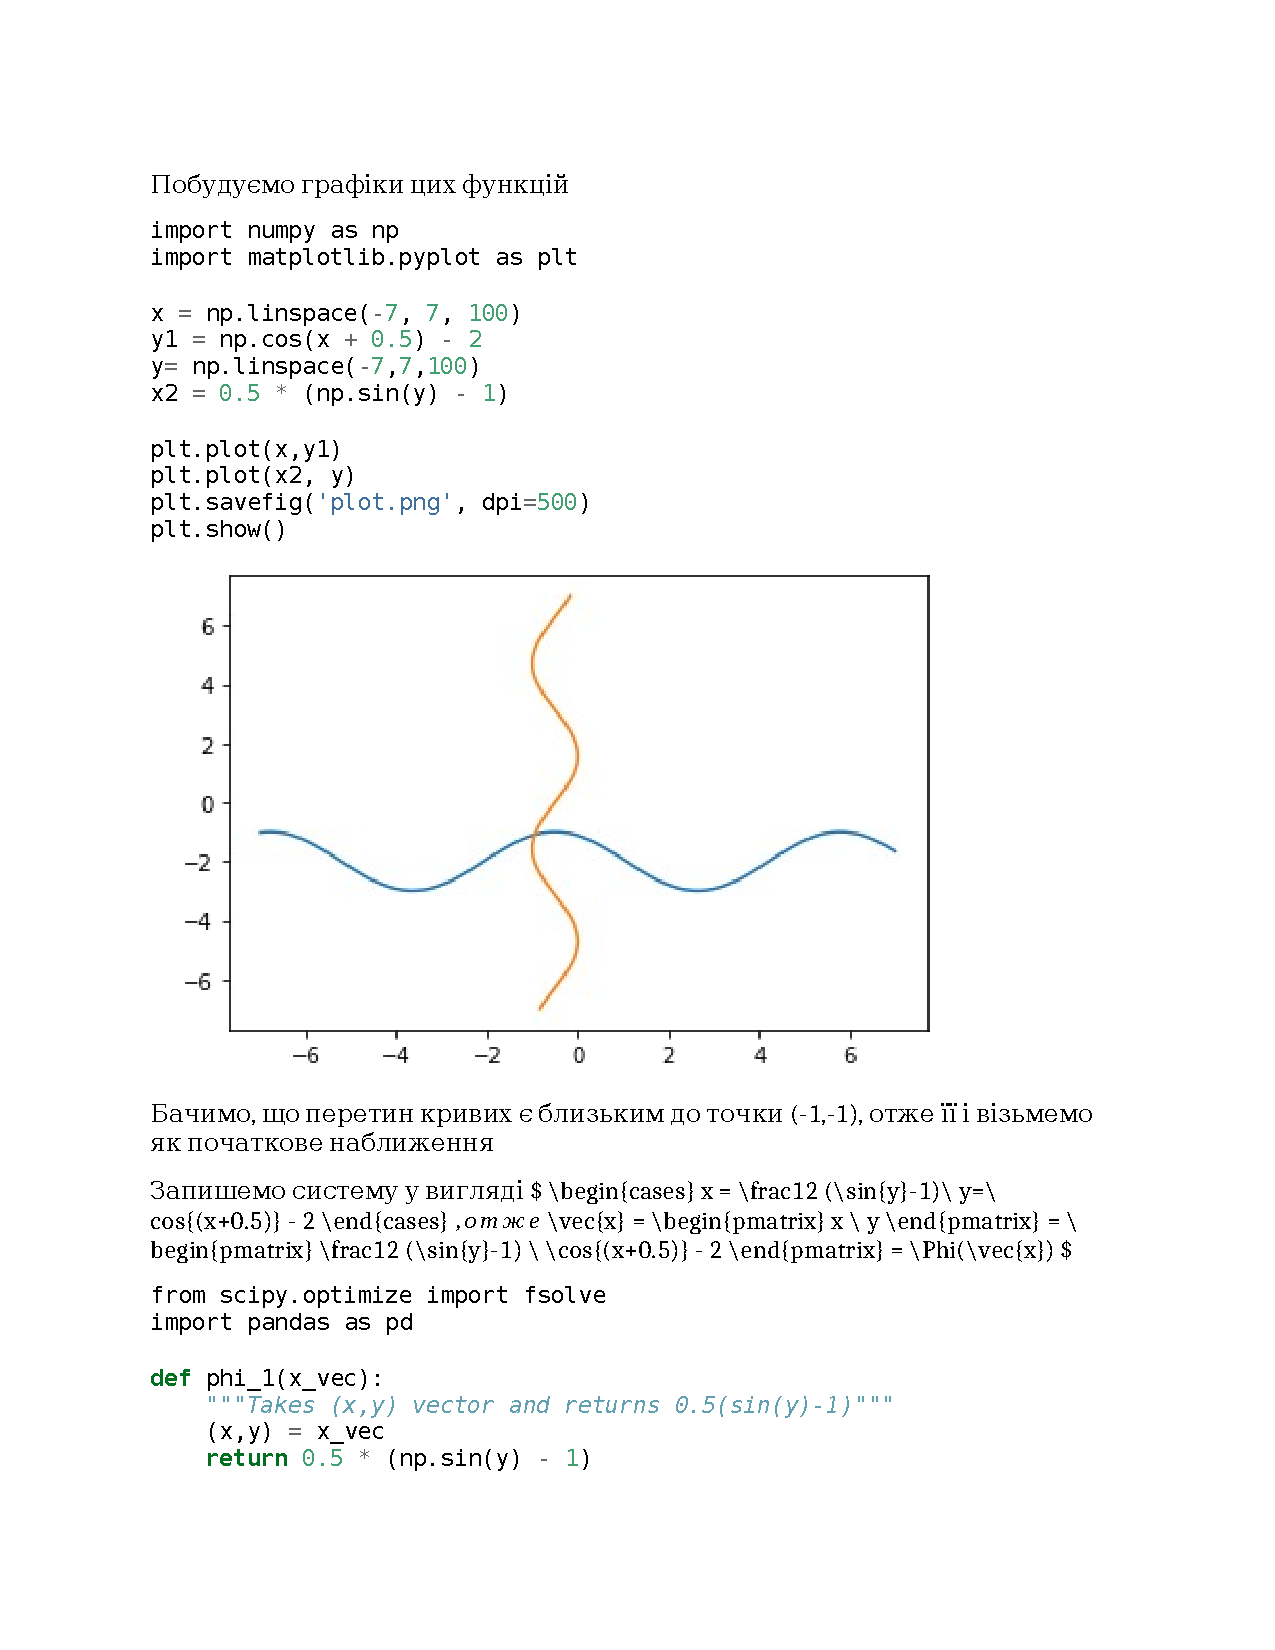
\includepdf[pages=-]{listing.pdf}

\end{document}


